\simplesection{Devops}

\begin{frame}{Git}    
    \begin{itemize}
        \item Git was used for version control during the complete Development
        \item GitLab at TU Berlin was used to host the repository as well as the bug tracker (\texttt{issues} on GitLab)
        \item Branching model was exhausted for automation of the build process by introducing a \texttt{deploy} branch which is queried periodically by \texttt{deneb}
        \item Development of different features or sub projects (scheduler, measurements, power saving, ...) was split across branches
    \end{itemize}
\end{frame}

\begin{frame}{GitLab}
	\begin{itemize}
		\item GitLab is a repository manager including an issue tracker and a wiki
		\item TU Berlin hosts a GitLab server with free, private projects for students
		\item GitLab offers \texttt{hooks} we use to trigger builds in Jenkins and kernel updates on \texttt{deneb}
		\item GitLabs \texttt{issues} have the advantage of being controllable via commit messages and hence were the better choice than redmine tickets
	\end{itemize}
\end{frame}

\begin{frame}{Jenkins}
	\begin{itemize}
		\item \textit{Jenkins CI} is an open source Continuous Integration Framework we used to automatically build the kernel
		\item runs on \texttt{zambezi}, a host within the local network
		\item each commit to the \texttt{master} branch of our repository triggers a compilation
		\item if compilation is successful, the current state of \texttt{master} branch is pushed to \texttt{deploy} branch
		\item successful and failing compilations trigger messages to our group chat
	\end{itemize}
\end{frame}

\begin{frame}{Polling on deneb}
	\begin{itemize}
		\item a cronjob on \texttt{deneb} is checking the \texttt{deploy} branch every 5 minutes for new versions
		\item if a newer version is found, it is pulled, compiled and installed
		\item logging is done to our group chat to alert on unforeseen behaviour
		\item new kernel is fed into \textit{GRUB} to be booted
	\end{itemize}
\end{frame}

\begin{frame}{GRUB on deneb}
	\begin{itemize}
		\item \textit{GRUB} on \texttt{deneb} is configured to once try to boot the newest kernel after its installation
		\item if kernel boot fails, \texttt{deneb} reboots with the second newest kernel available
		\item if booting succeeds, the newest kernel is chosen as default
		\item in all cases, logging to our group chat is ensured
		\item for debugging non-bootable kernels, we installed a serial line to \texttt{zambezi}
	\end{itemize}
\end{frame}

\begin{frame}
	\begin{figure}[h]
		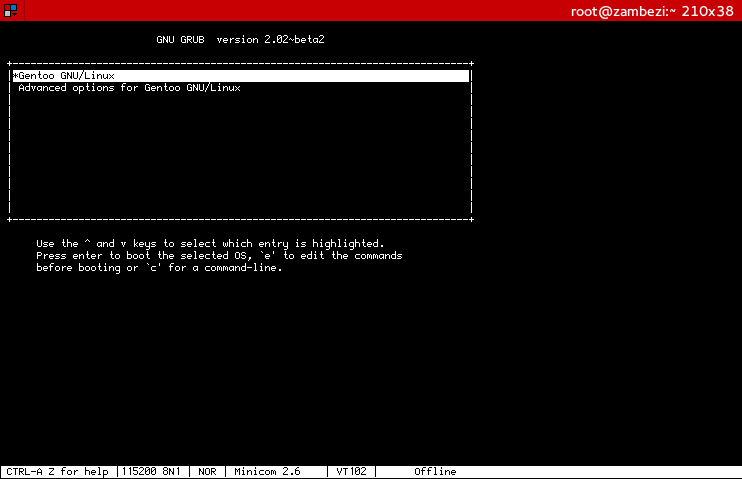
\includegraphics[width=.8\textwidth]{img/serialGRUB.png}
		\caption{GRUB boot choices over minicom on \texttt{zambezi}}
		\label{fig:serialGRUB}
	\end{figure}
\end{frame}

\begin{frame}{QEMU I}
	\begin{itemize}
		\item to test if kernels boot before pushing them to master, an easy-to-use script spawning a QEMU VM was written
		\item central problem was there needs to be a rootfs along with the kernel image for QEMU to be able to boot the kernel
		\item busybox and some base files were crafted together to form a rootfs, whole build is scripted
	\end{itemize}
\end{frame}

\begin{frame}{QEMU II}
	\begin{itemize}
		\item boot-testing opened up the possibility to include userspace tools in the initramfs and hence QEMU was used to debug them too
		\item this setup is also used to simulate the VM that are to be scheduled on \texttt{deneb}
		\item for future work, if one would configure QEMU to emulate a specific processor, the power sub system coud be debugged in QEMU too
		\item \texttt{deneb} would just be needed for measurements
	\end{itemize}
\end{frame}
